\section{时间隐通道检测方法}
\label{chap:backinfo:detect}

%本节主要介绍,现有的时间隐通道检测方法,主要包括哪些
时间隐通道的发展,催生了新的时间隐通道检测技术。基于统计及分布一致性进行时间隐通道检测,是通常使用的检测方法。在某些应用场景中,基于标准差的检测方法,以及基于机器学习的检测方法也是有效的。\nupcite{ARCHIBALD2014284}

\subsection{基于分布曲线的检测方法}
\label{chap:backinfo:detect:statistical}

%统计看CDF差异,主要评估了哪些参数
传输过程中的时间特征,是时间隐通道检测方法的检测目标,通常检测的对象为IPD。对于IPD来说,如果传输延迟恒定,则发送方观测到的IPD与接收方观测到的IPD是一致的。然而,当网络噪声或者时间隐通道存在时,IPD统计出现偏离。监听者检测时间隐通道,需要对比分布之间的最大偏离程度,根据分布的偏离情况判断是否存在隐通道。

\insertEquation{
    \begin{equation}
    \label{equ:2:ks}
		D_{KS}\ =\ sup_{x}\ |F_{1,\ n}(x)\ -\ G_{1,\ m}(x)|
    \end{equation}
    \begin{equation}
    \label{equ:2:ks-p}
        D_{KS,\ 0.05}\ =\ 1.358\ \times\ \sqrt{\frac{n\ +\ m}{n\ \times\ m}}
    \end{equation}
}

\insertFigure{
	\begin{figure}
		\centering
        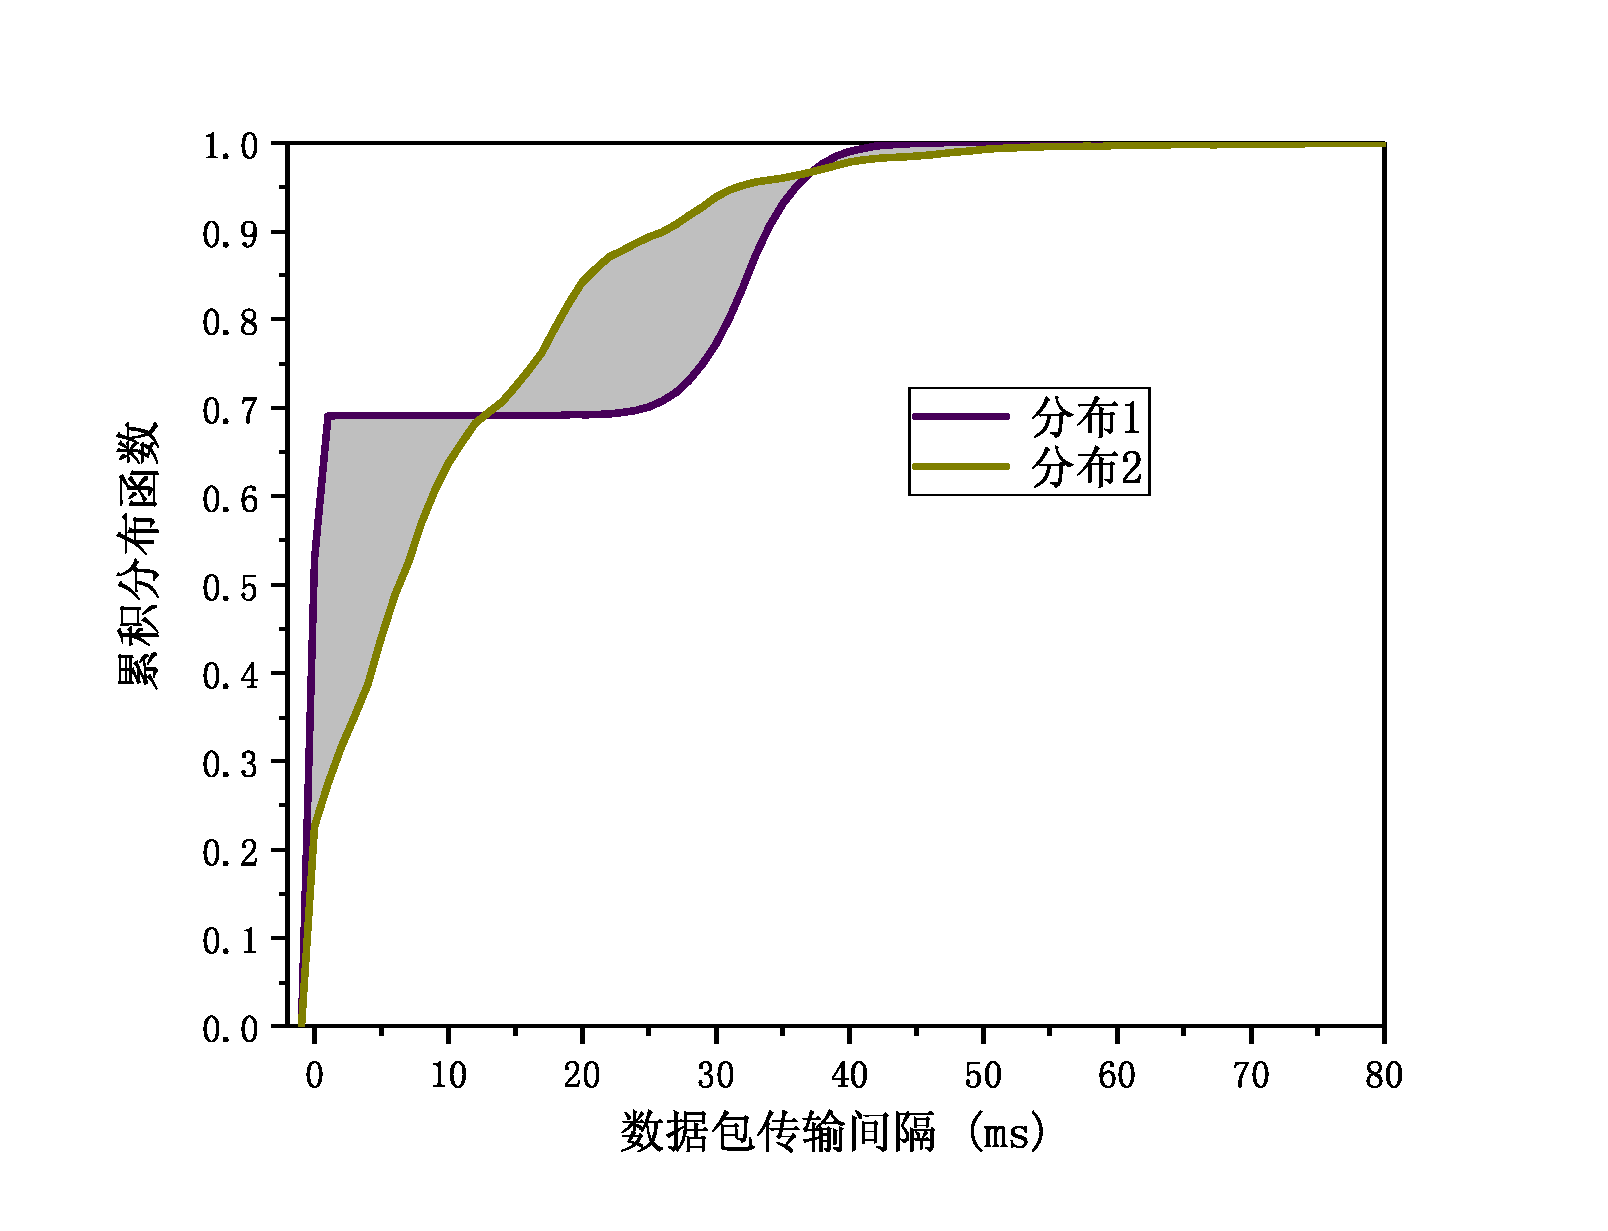
\includegraphics[width=0.8\textwidth]{chapters/chapter2/figures/ks-cdf.pdf}
        \caption{CDF曲线差异示意图}\label{fig:2:ks-cdf}
	\end{figure}
}

%如何根据差异,判断一致性
如图\nref{fig:2:ks-cdf},两条不同的CDF曲线,分别代表不同的IPD分布。通过公式(\nref{equ:2:ks}),计算CDF曲线差异绝对值的最大值,得到分布曲线之间的直接差异。根据一致性假设理论,进行K-S检验的两个样本,在{95\ \%}一致的假设前提下,通过公式(\nref{equ:2:ks-p})计算置信值$D_{KS,\ 0.05}$。当$D_{KS,\ 0.05}>D_{KS}$时,即可判定$F_{1,\ n}$与$G_{1,\ m}$属于相同分布。

除了K-S检验外,常用的双样本检验方法还包括{Welch's\ \ t检验}、Epps-Singleton检验、Mann-Whitney rank检验及Wilcoxon rank检验等。不同的检验方法有适用的分布类型,在使用中需要与检测对象相对应。当检测样本与参照样本通过了检验,则证明二者在分布方面没有明显差异,存在隐通道的概率较小。

\subsection{基于熵的检测方法}
\label{chap:backinfo:detect:entropy}

%计算熵,判断的对象是什么
数学统计中,Kullback–Leibler散度又称相对熵,是一种判断概率质量函数差异的方法。在实际应用中,通过计算样本之间熵值大小,判断分布之间的一致性。\nupcite{5590253,Gianvecchio:2007:DCT:1315245.1315284,Cabuk:2004:ICT:1030083.1030108,6296078}

\insertEquation{
    \begin{equation}
    \label{equ:2:kld}
		D_{KL}(F(x)\ ||\ G(x))\ =\ \sum_{x=i}\ f(x)\ \times\ \log \frac{f(x)}{g(x)}
	\end{equation}
}

\insertTable{
	\begin{table}
        \centering
        \caption{IPD的概率质量函数示意表}
        \label{tab:2:pmf-dis}
        \begin{tabular*}{0.6\textwidth}{@{\extracolsep{\fill}}ccc}
        \toprule
        IPD & f(x) & g(x)\\ 
        \midrule
        0 & 0.52921 & 0.2265 \\ 
        1 & 0.16155 & 0.04827 \\ 
        2 & 0.00075 & 0.04231 \\ 
        3 & 0.00011 & 0.03467 \\ 
        4 & 0.00002 & 0.03603 \\ 
        5 & 0.00002 & 0.05287 \\ 
        \bottomrule
        \end{tabular*}
    \end{table}
}

如表\nref{tab:2:pmf-dis}所示,概率质量函数PMF(Probability Mass Function)对应的是不同IPD的统计概率,参照分布的概率函数为$g(x)$,样本分布的概率函数为$f(x)$。通过公式(\nref{equ:2:kld})计算$D_{KL}$,得到结果$0.278$,高于检测阈值$0.1$\nupcite{ZHANG201866},因此得出结论,样本与参照分布不一致,隐通道存在概率较高。

\insertTable{
	\begin{table}
        \centering
        \caption{经典时间隐通道的检验准确率}
        \label{tab:2:test-results}
        \begin{tabular*}{0.6\textwidth}{@{\extracolsep{\fill}}cccc}
        \toprule
        检验方法 & JitterBug\nupcite{shah2006keyboards} & TR-CTC\nupcite{Cabuk:2004:ICT:1030083.1030108} & MB-CTC\nupcite{10.1007/978-3-642-16435-4_15} \\ 
        \midrule
        K-S检验 & 0.66 & - & 0.56 \\
        T检验 & 0.86 & 0.56 & 0.95 \\
        K-L散度 & 0.62 & 0.56 & 0.65 \\
        \bottomrule
        \end{tabular*}
    \end{table}
}

如表\nref{tab:2:test-results},对于几种经典的时间隐通道,在SSH场景中不同检验方法的准确率存在差异。\nupcite{ARCHIBALD2014284}由于TR-CTC不改变传输特征,因此通过K-S检验及T检验效果准确率较低。K-L散度对概率变化更敏感,计算过程不仅考虑了概率本身,概率所占的比重也同时纳入计算。结果对比可以发现,通过结合不同的检测方式,能够实现原理上的互补,具有更好的检测效果。

\subsection{基于机器学习的检测方法}
\label{chap:backinfo:detect:machine}

%机器学习的模型是怎样生成的
基于机器学习的时间隐通道检测方法,需要预先获取宿主信道的传输特征,然后根据传输特征训练对应的模型。对于监听者,基于统计的时间隐通道检测方法针对的是特定隐通道,并且在获取足够的统计数据后才具有较好效果。基于机器学习的时间隐通道检测方法,在模型训练完成后,具备传输中实时监测能力,并且不限定隐通道类型。\nupcite{8875875,7087364}

%判定结果如何认定是否通过
基于SVM(Support Vector Machines)的检测方法,通过提取样本中的特征向量,用于训练SVM的分类器。识别过程中,提取检测样本中的指纹特征,通过训练过的SVM进行分类判断。用于训练的数据集,需要在已知时间隐通道的基础上,生成各种隐通道的传输特征,计算其K-S结果、K-L散度及统计规律等特征。\nupcite{7087364}基于SVM检测方法,在盲测情况下具有较好的效果,对于传输特征稳定的信道来说,具备良好的检测结果。

在VoLTE视频通话中,语音信道具有明确的规律性,现有的检测方法均可实现准确判别。然而,对于视频信道,网络噪声与传输需求存在不确定性,无法提取出明确的传输特征。因此,要检测出VoLTE视频信道中的时间隐通道,无法以局部传输特征代替全局特征,需要在一定规模的统计数据基础上进行检验。